\documentclass[a4paper]{jarticle}
\usepackage{sf}

%図に関する設定
\usepackage[dvipdfmx]{graphicx}
\graphicspath{{0.Fig/}}
\renewcommand{\figurename}{Fig.}
%数式に関する設定
\usepackage{amsmath}
%添削時の色の設定%{\color{red} 赤色の文字}で使う
\usepackage{xcolor} 

\title{センシングフォーラム予稿テンプレート}
\author{○金谷 孝一郎$^1$, 村上 健一$^2$, 山川 雄司$^3$}
\affiliation{
$^1$ 東京大学,
$^2$ 東京大学,
$^3$ 東京大学 }
\Etitle{Template for proceedings of Sensing Forum}
\Eauthor{○Koichiro Kanaya , Kenichi Murakami and Yuji Yamakawa  }
\Eaffiliation{
$^1$ University of Tokyo,
$^2$ University of Tokyo,
$^3$ University of Tokyo }
\Abstract{日本語アブストラクト(本文が英語の場合は英語でも可).
200字程度で記載.
〇〇〇〇〇〇〇〇〇〇〇〇〇〇〇〇〇〇〇〇〇〇〇〇〇〇〇〇〇〇〇〇〇〇
〇〇〇〇〇〇〇〇〇〇〇〇〇〇〇〇〇〇〇〇〇〇〇〇〇〇〇〇〇〇〇〇〇〇
〇〇〇〇〇〇〇〇〇〇〇〇〇〇〇〇〇〇〇〇〇〇〇〇〇〇〇〇〇〇〇〇〇〇
〇〇〇〇〇〇〇〇〇〇〇〇〇〇〇〇〇〇〇〇〇〇〇〇〇〇〇〇〇〇〇〇〇〇
〇〇〇〇〇〇〇〇〇〇〇〇〇〇〇〇〇〇〇〇〇〇〇〇〇〇〇〇〇〇〇〇〇〇
}
\begin{document}
\maketitle
\iffalse
\section{原稿の書き方}
\begin{itemize}
\item 原稿枚数はA4版で4~6ページです.超過しないようご注意下さい.
\item 用紙余白は上下24mm,左右15mmとし,本文を縦250mm×横180mmの枠内に収めて下さい.
\item 冒頭に以下の項目を書いてください.
\begin{itemize}
\item 一行目:和文題目.
\item 二行目:和文著者名.登壇者の前に必ず○をつけてください.
\item 三行目:和文所属名.
\item 四行目:英文題目.
\item 五行目:英文著者名.登壇者の前に必ず○をつけてください.
\item 六行目:英文所属名.
\item 七行目以降:要旨(日本語.論文の本文が英文の場合,英語でも結構です)
\end{itemize}
\item 原稿はPDF形式で作成してください.印字の正確性を期すため,PDFファイル作成時にフォントの埋め込みをお願い致します.
\item 引用は文献\cite{ref1}のように記載してください.
\end{itemize}
\begin{thebibliography}{9}
\bibitem{ref1}
計測 太郎:センシングフォーラム予稿の書き方,
第39回センシングフォーラム論文集,pp. 1-5, 2022.
\end{thebibliography}
\section{図の挿入例}
以下にPDF形式の図を挿入します。

\begin{figure}[htbp]
    \centering
    \includegraphics[width=0.5\textwidth]{example.pdf}
    \caption{サンプル図}
    \label{fig:sample}
\end{figure}

図~\ref{fig:sample}はサンプル図です。
\fi

%%%%%%%%%%%%%%%%%%%%%%%%%%%%%%%%%%%%%%%%%%%%%%%%%%%%%%%%%%%%%%%%%%%%%%%%%%%%%%%%%%%%%%%%%%%%%%%%%%%%%%%%%%%%%%%%%%%%%%%%%%%%%%%%%%%%%%%%%%%%%%%%%%%%%
\section{緒言}
近年,医療分野では患者と医師双方にメリットがあるとして,低侵襲手術が注目されている.従来の開腹手術と比較し,低侵襲手術は小さな皮膚切開を介して手術を行う.
これにより,患者にとっては手術リスクや感染症リスクの低下や入院期間,回復期間の短縮といったメリットがある.また,外科医にとっても手術時の肉体的疲労の低減や,x線透視装置を用いた手術においては,放射線被曝の低減といったメリットがある.

しかし,低侵襲手術にもちいられる鉗子グリッパは,スペース的な制約や生体適合性の需要から,力センサを搭載することが難しい.この力センサの不在は,外科医の練習期間の長期化や,ロボットによる自動化を推進する上での課題となっている.
鉗子グリッパへの力センサ搭載が困難である主な要因は,その小型化,生体適合性,殺菌処理への耐久性にある.鉗子グリッパ内の限られた空間内では,力センサとその計測に必要な配線を組み込む物理的なスペースが不足する.また,力センサが必ずしもチタンや
ステンレスといった生体適合素材で構成されるとは限らない.さらに,鉗子グリッパは高温の蒸気により殺菌され,数回の殺菌処理によりセンサの精度が低下する.これらの要因による力センサの不在を解決するために,鉗子グリッパに搭載可能な力センサの開発や,
力センサを用いないで接触力を推定する研究が行われている.%おり,本研究は後者に該当する.

センサはリアルタイムの触覚フィードバックに使用され,ロボットによる手術の自動化では,最低0.5 kHz,理想的には,1 kHzの更新頻度が必要とされる.
要求される更新頻度を満たすためには,反力推定では計算効率の高いアルゴリズムである必要があり,本研究では,臓器等の柔軟物をバネとダンパでモデル化し,バネ定数と粘性減衰係数を同定し,反力推定を行う.

\section{関連研究}
センサを用いないで反力を推定する研究は,大きく2つ,1;内視鏡画像から反力を推定する研究,2;駆動用モータやワイヤから反力を推定する研究に分類できる.
まず,画像ベースの研究に関して,
ChuaらはRGB画像とロボットの状態をニューラルネットワークの入力とすることで,画像のみやロボットの状態のみを入力とする場合より,汎化能力を向上させた.さらに,単一フレームごとに反力を推定することで,37.7 Hzの更新速度を達成し,
リカレントニューラルネットワーク(12.4 Hz)と比較して,高速な反力推定を実現した.しかし,学習系を用いた手法では,1 kHzの更新頻度を達成することが難しいと考える.
Wangらは変形前後の画像から変位を計測し,既知の材料特性と有限要素法を用いて,力の位置と大きさを推定した.変位の推定精度が反力推定精度に影響し,高制度な変位計測には,マーカが必要となるという課題がある.
次に,駆動用モータやワイヤから推定する研究に関して,
Xueらは,ワイヤ駆動する鉗子グリッパをケーブルプーリーシステムでモデル化し,張力伝達特性,エンドエフェクタのカップル特性,隣接するプーリーの摩擦特性を考慮し,鉗子の把持力を推定した.しかし,グリッパが停止しているときの把持力は停止前の
値を取り続けるアルゴリズムであり,塑性変形が進む柔軟物の反力を推定することは難しいと考える.

さらに,柔軟物をモデル化しロボットで操作する研究は,大きく柔軟物のモデル化に関して3つに分類できる.
1;柔軟物をバネとダンパでモデル化する研究,2;柔軟物を有限要素法でモデル化する研究,3;Position Based Dynamics(PBD)でモデル化する研究である.
まず,バネとダンパによりモデル化する手法は,計算量が少ない一方で,柔軟物の変形に対するモデルの精度が低い手法である.しかし,モデルのパラメータを同定する上で,柔軟物全体の変形を計測するだけでよいので内視鏡画像やグリッパのエンコーダによる計測
が可能である.
次に,有限要素法でモデル化する手法は,柔軟物の変形に対するモデルの精度が高い一方で,計算量が多く,リアルタイムでの反力推定には不向きであり,密度やヤング率,ポアソン比を事前に計測する必要がある.
最後に,PBDでモデル化する手法は,柔軟物の変形に対するモデルの精度はバネダンパより高く,計算量は有限要素法よりも少ない.しかし,柔軟物のせん断変形を計測する必要があり,マーカが必要となるが,臓器が出血することを考慮すると画像計測は難しいと考える.

本研究では,柔軟物をバネとダンパでモデル化し,グリッパの目標位置に到達した際の柔軟物の変形量を推定する.



\section{課題設定}
グリッパに力センサを搭載しない場合,グリッパが目標位置に到達した際に,力入力は,0 [N]になるが,柔軟物からの反力は存在し,塑性変形が進行するにしたがって,柔軟物からの反力は減少する.
本研究では,柔軟物の変形と反力の関係をバネとダンパを用いてモデル化し,グリッパの目標位置に到達した際の柔軟物の変形量を推定することを目的とする.
\section{提案手法}
一般に,弾性と粘性の挙動を表現するには,バネとダンパの要素が4つ必要である\cite{?}.4つの要素を用いた場合の組み合わせは,7種類存在し,リアルタイムで同定している研究\cite{??}と
比較するために,図~\ref{?}を用いる.図~\ref{?}のモデルの接触力$f$と,変形量$x$の関係は以下のように表される.
\begin{equation}
    % \frac{k_1 k_2}{c_2}\int{x}\,dt + k_1 x = \frac{k_1k_2}{c_1 c_2}\iint{f}\,dt\,dt + \frac{k_1}{c_2}(1+\frac{k_2}{k_1}+\frac{c_2}{c_1})\int{f}\,dt + f
p_1 {x} + p_2 \int{x}\,dt = p_3\int{f}\,dt +p_4\iint{f}\,dt\,dt  + f
\label{eq:BSmodel}
\end{equation}
% \begin{equation}
%     \begin{aligned}
%         \frac{k_1 k_2}{c_2} \int{x}\,dt + k_1 x &= 
%         \frac{k_1 k_2}{c_1 c_2} \iint{f}\,dt\,dt \\
%         &\quad + \frac{k_1}{c_2} \left( 1 + \frac{k_2}{k_1} + \frac{c_2}{c_1} \right) \int{f}\,dt + f
%     \end{aligned}
%     \label{eq:BSmodel}
% \end{equation}
% ここで,
% \begin{equation}
%     \begin{aligned}
%         a_1 &= \frac{c_1 c_2 (k_1 + k_2)}{k_1 k_2}      \\
%         a_2 &= c_1  \\
%         b_1 &= \frac{c_1 c_2}{k_1 k_2} \\
%         b_2 &= \frac{c_1 k_2 + c_2 k_1 + c_2 k_2}{k_1 + k_2} \\
%     \end{aligned}
% \end{equation}
ここで,
\begin{equation}
    \begin{aligned}
        p_1 &= k_1,  \\
        p_2 &= \frac{k_1 k_2}{c_2},    \\
        p_3 &= \frac{k_1}{c_2}\left(1+\frac{k_2}{k_1}+\frac{c_2}{c_1}\right),\\
        p_4 &= \frac{k_1k_2}{c_1 c_2} \\
    \end{aligned}
    \label{eq:p2ck}
\end{equation}
である.$k_1$,$k_2$は弾性係数であり,$c_1$,$c_2$は粘性減衰係数である.
接触力$f$は,モータの力入力を用い,変形量$x$は,グリッパの目標軌道を用いて,$p_1$,$p_2$,$p_3$,$p_4$を同定し,$k_1$,$k_2$,$c_1$,$c_2$を求める.
式~(\ref{eq:BSmodel})をタイムステップを行に格納し,行列形式で表すと以下のようになる.
\begin{equation}
    \mathbf{M}\mathbf{p} = \mathbf{q} 
    \label{eq:Mp_q}
\end{equation}
ただし,
\begin{equation}
    \begin{aligned}
        \mathbf{M} &= \begin{bmatrix}
            \boldsymbol{x}, & \int{\boldsymbol{x}}, & -\int{\boldsymbol{f}}, & -\iint{\boldsymbol{f}}\\
        \end{bmatrix}, \\
        \mathbf{p}  &= \begin{bmatrix}
            p_1 \\
            p_2 \\
            p_3 \\
            p_4
        \end{bmatrix}, \quad\quad\quad\quad
        \mathbf{q}   = \boldsymbol{f}
    \end{aligned}
\label{eq:BSmodel_matrix}
\end{equation}
である.
粘弾性係数$k_1$,$k_2$,$c_1$,$c_2$を同定することは,行列$\mathbf{M}$の擬似逆行列を算出する問題に帰着する.
% しかし,エンコーダのノイズや,そのノイズが{\color{red} 制御係数倍}され,モータの力入力に現れる.これらのノイズにより粘弾性係数の同定精度が低下する課題がある.
しかし,エンコーダの計測結果には,ノイズが含まれ,位置制御するモータの力入力には,{\color{red} 制御係数倍}されたノイズが現れる.
このノイズにより粘弾性係数の同定精度が低下するという課題がある.

この課題を解決するために,まず,\ref{subsec:QR_traj_and_calculation}節では,行列$\mathbf{M}$の特異値に着目し,
ノイズにロバストなグリッパの軌道生成方法と,その軌道に適した計算方法について述べる.
次に,\ref{subsec:downsample}節では,粘弾性係数が0や無限大に近づくことを防ぐために,グリッパの軌道からデータを抽出する方法について述べる.

\subsection{特異値分解を用いたグリッパの軌道生成と軌道に適した同定計算}\label{subsec:QR_traj_and_calculation}
グリッパの軌道生成において,特異値分解を用いることで,ノイズにロバストな軌道を生成する.ノイズを明示的に扱うために,$\mathbf{q}$のノイズを$\mathbf{noise}$とし,
$\mathbf{p}$を算出する式変形は,行列$\mathbf{M}$の擬似逆行列を算出し,
\begin{equation}
    \begin{aligned}
    \mathbf{M}\mathbf{p} &= \mathbf{q} + \mathbf{noise}\\
              \mathbf{p} &= \mathbf{M}^{\dagger}(\mathbf{q} + \mathbf{noise})\\ 
              \mathbf{p} &= \sum \frac{1}{\gamma}vu^T(\mathbf{q}+\mathbf{noise})\\
    \end{aligned}     
\end{equation}
のようになる.ここで,$\gamma$は行列$\mathbf{M}$の特異値であり,$O(\min({\mathbf{p}}))\gg\frac{O(\mathbf{noise})}{O(\mathbf{\gamma})}$のように$\gamma$を決定することで
ノイズの影響を抑えることができる.

次に,行列$\mathbf{M}$をQR分解し,$\mathbf{Q}$と$\mathbf{R}$を独立して生成することで,$\mathbf{M}$の特異値と1列目のグリッパの軌道を任意に決定する.
QR分解を用いた$\mathbf{M}$の生成方法を図~\ref{QR分解}に示す.
% $\mathbf{M}$の特異値の大きさを任意に決定し,グリッパの軌道である$\mathbf{M}$の1列目はグリッパが追従しやすい5次関数形状にする.

対角行列$\mathbf{R}$は,上記でパラメータ$\mathbf{p}$の最小値と$\mathbf{noise}$のオーダを考慮して決定した$\gamma$を対角成分とした$4\times4$行列である.

直交行列$\mathbf{Q}$は,図~\ref{QR分解}の上側ルートで生成される.
1サイクル前に同定したパラメータ$\mathbf{p}$を柔軟物モデルに適応し,仮想的な5次関数形状の変形$x$を与えることで一時的な行列$\mathbf{M}_{\mathrm{temp}}$を生成し,QR分解することでQを得る.
最終的に,独立して得られて$\mathbf{Q}$と$\mathbf{R}$を掛け合わせることで,行列$\mathbf{M}$を生成し,その1列目をグリッパの軌道とする.

このグリッパの軌道生成に適したパラメータ$\mathbf{p}$の計算方法について述べる.粘弾性モデルの変形と反力の関係式~(\ref{eq:BSmodel})を行列形式である式~(\ref{eq:BSmodel_matrix})に変形する際,
$\mathbf{q}$は$\boldsymbol{x} , \int{\boldsymbol{x}} , \int{\boldsymbol{f}} , \iint{\boldsymbol{f}}$の5通りの選び方がある.上記で述べたグリッパの軌道は,$\mathbf{q}$のノイズの影響を抑える軌道になっており,
$\mathbf{q}$にもっともノイズの大きい$\boldsymbol{f}$を用いることで
提案した軌道生成が有効に働く.
\subsection{粘弾性係数の妥当性を向上させるためのデータの抽出}\label{subsec:downsample}
式~(\ref{eq:Mp_q})は不能であり,求める解$\mathbf{p}$が4要素であるのに対し,方程式の数が過剰であり矛盾する式が含まれる.一部の矛盾する式より粘弾性係数が負になり,物理的に妥当性を失う.
そこで,式~(\ref{eq:Mp_q})の擬似逆行列の算出方法を逐次的に行い,粘弾性係数が物理的に妥当でないデータは除外する.
まず,擬似逆行列の逐次的な算出方法について述べる.タイムステップが$n-1$までの行列$\mathbf{M}$を$\mathbf{M}_{n-1}$とし,$n$番目のタイムステップのデータ$\mathbf{m}_n$として,タイムステップ$n$での行列$\mathbf{M}_n$を,
\begin{equation}
    \begin{aligned}
        \mathbf{M}_n &= \begin{bmatrix}
            \mathbf{M}_{n-1} \\
            \mathbf{m}_n
        \end{bmatrix},\\
        \mathbf{m_{n}}&=\begin{bmatrix}
            x_{n} & \int{x_{n}} & -\int{f_{n}}\ & -\iint{f_{n}}\\
        \end{bmatrix}
    \end{aligned}
\end{equation}
とする.このとき$(\mathbf{M_{n}}^{T}\mathbf{M_{n}})^{-1}$を$\mathbf{J}_{n}$とし,$\mathbf{J}_{n}$の更新式はWoodburyの公式を用いて,
\begin{equation}
    \begin{aligned}
    \mathbf{J}_n &= (\mathbf{M_{n}}^{T}\mathbf{M_{n}})^{-1}\\
                 &= (\mathbf{M_{n-1}}^{T}\mathbf{M_{n-1}} + \mathbf{m_{n}}^{T}\mathbf{m_{n}})^{-1}\\
                 &= \mathbf{J}_{n-1} - \frac{\mathbf{J}_{n-1}\mathbf{m_{n}}\mathbf{m_{n}}^{T}\mathbf{J}_{n-1}}{1+\mathbf{m_{n}}^{T}\mathbf{J}_{n-1}\mathbf{m_{n}}}
    \end{aligned}
    \label{eq:step_J}
\end{equation}
と表せる.$\mathbf{p}$の$n-1$番目と$n$番目の関係は,
\begin{equation}
    \begin{aligned}
    \mathbf{p}_n &= (\mathbf{M_{n}}^{T}\mathbf{M_{n}})^{-1}\mathbf{M_{n}}^{T}\mathbf{q_{n}}\\
                 &= \mathbf{J}_{n}\mathbf{M_{n}}^{T}\mathbf{q_{n}}\\
                 &= \mathbf{J}_{n}(\mathbf{p}_{n-1}+\mathbf{m_{n}}^{T}\mathbf{q_{n}})\\
    \end{aligned}
    \label{eq:step_p}
\end{equation}
となる.この更新式~(\ref{eq:step_J}),~(\ref{eq:step_p})とタイムステップ$n$で計測されたデータ$\mathbf{m_{n}}$と$\mathbf{q_{n}}$を用いて$\mathbf{p}_{n\_temp}$を算出し,$\mathbf{p}$の更新に利用するか,除外するか判断する.

次に,除外するデータの決定方法について述べる.式~(\ref{eq:p2ck})を変形し$\mathbf{p}$から$k_1$,$k_2$,$c_1$,$c_2$は,
\begin{equation}
    \begin{aligned}
        k_1 &= p_1 ,\\
        k_2 &= \frac{p_2}{p_3 - \frac{p_4 p_1}{p_2} - \frac{p_2}{p_1}} ,\\
        c_1 &= \frac{p_2}{p_4},\\
        c_2 &= \frac{p_1}{p_3 - \frac{p_4 p_1}{p_2} - \frac{p_2}{p_1}} 
    \end{aligned}
\end{equation}
のように算出できる.さらに,更新に用いる$\mathbf{p}_{n\_temp}$の条件は,
\begin{equation}
    \begin{aligned}
        10^{-7} < \mathbf{p}_{n} < 10^{7} ,\\
        10^{-7} < \left( p_3 - \frac{p_4 p_1}{p_2} - \frac{p_2}{p_1} \right)
    \end{aligned}
\end{equation}
とした.

\section{評価実験}
\subsection{実験システム}
実験に用いたグリッパを図~\ref{fig:setup}に示す.駆動系にはシャフトモータ(...),ドライバ(Panasonic製,MADHT1107L01)を用いた.
本システムは1 kHzの制御周期で動作した.
windows PC上でグリッパの軌道を生成し,シリアル通信(RS422,ボートレート...)でdSPACE DS1104に送信し,dSPACEがシステム全体のリアルタイム制御を管理した.
反力の真値を確認するために,力センサ(レプトリノ社製,...)を用いた.
研修医の超音波ガイド下での処置の練習対象として,鶏むね肉や,豆腐,ゼラチンを用いられ,縫合の練習対象としてバナナを用いている場合があることから\cite{?}\cite{?}\cite{?},
実験対象として,鶏むね肉,豆腐,ゼラチン,バナナを用いた.
\subsection{評価方法}
実験では,6秒間対象物を変形させ,その後9秒間一定の目標位置を与えた.変形過程の6秒間で柔軟物モデルのパラメータ($k_1, k_2, c_1, c_2$)を同定し,目標位置が一定の9秒間での反力を推定した.
推定反力は力センサの計測結果との平均絶対誤差(MAE: Mean Absolute Error)を算出し評価した.
実験では,2つのグリッパ軌道により反力推定精度を比較した.1つは,提案手法により生成したグリッパ軌道であり,もう1つは,それと同じ最終値を持つ5次関数形状の軌道である.5次関数の境界条件は,....
\subsection{結果}
\begin{figure}[htbp]
    \centering
    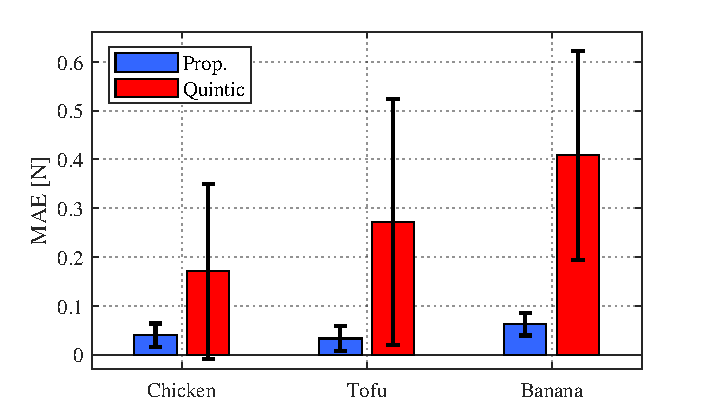
\includegraphics[width=0.5\textwidth]{bar_result.pdf}
    \caption{サンプル図}
    \label{fig:bar_result}
\end{figure}
〇〇〇〇〇〇〇〇〇〇〇〇〇〇〇〇〇〇〇〇〇〇〇〇〇〇〇〇〇〇〇〇〇〇
〇〇〇〇〇〇〇〇〇〇〇〇〇〇〇〇〇〇〇〇〇〇〇〇〇〇〇〇〇〇〇〇〇〇
〇〇〇〇〇〇〇〇〇〇〇〇〇〇〇〇〇〇〇〇〇〇〇〇〇〇〇〇〇〇〇〇〇〇
〇〇〇〇〇〇〇〇〇〇〇〇〇〇〇〇〇〇〇〇〇〇〇〇〇〇〇〇〇〇〇〇〇〇
\begin{figure}[htbp]
    \centering
    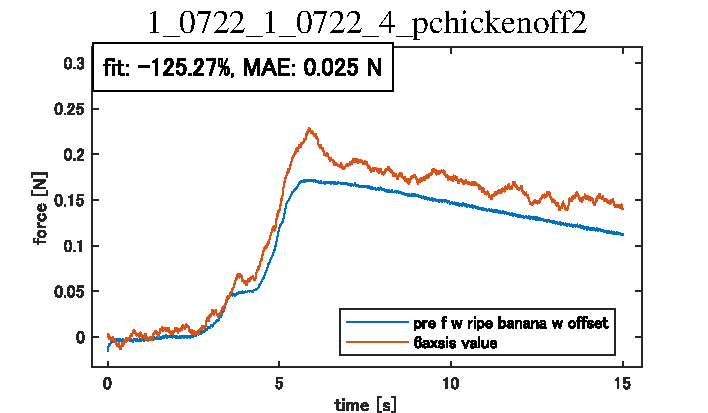
\includegraphics[width=0.5\textwidth]{test.pdf}
    \caption{サンプル図}
    \label{fig:twst}
\end{figure}
〇〇〇〇〇〇〇〇〇〇〇〇〇〇〇〇〇〇〇〇〇〇〇〇〇〇〇〇〇〇〇〇〇〇
〇〇〇〇〇〇〇〇〇〇〇〇〇〇〇〇〇〇〇〇〇〇〇〇〇〇〇〇〇〇〇〇〇〇
〇〇〇〇〇〇〇〇〇〇〇〇〇〇〇〇〇〇〇〇〇〇〇〇〇〇〇〇〇〇〇〇〇〇
〇〇〇〇〇〇〇〇〇〇〇〇〇〇〇〇〇〇〇〇〇〇〇〇〇〇〇〇〇〇〇〇〇〇
〇〇〇〇〇〇〇〇〇〇〇〇〇〇〇〇〇〇〇〇〇〇〇〇〇〇〇〇〇〇〇〇〇〇

〇〇〇〇〇〇〇〇〇〇〇〇〇〇〇〇〇〇〇〇〇〇〇〇〇〇〇〇〇〇〇〇〇〇
〇〇〇〇〇〇〇〇〇〇〇〇〇〇〇〇〇〇〇〇〇〇〇〇〇〇〇〇〇〇〇〇〇〇
〇〇〇〇〇〇〇〇〇〇〇〇〇〇〇〇〇〇〇〇〇〇〇〇〇〇〇〇〇〇〇〇〇〇
〇〇〇〇〇〇〇〇〇〇〇〇〇〇〇〇〇〇〇〇〇〇〇〇〇〇〇〇〇〇〇〇〇〇
〇〇〇〇〇〇〇〇〇〇〇〇〇〇〇〇〇〇〇〇〇〇〇〇〇〇〇〇〇〇〇〇〇〇
\end{document}

% end of sftemplate.tex